\documentclass[12pt,a4paper]{article}
\usepackage[utf8x]{inputenc}
\usepackage{ucs}
\usepackage[MeX]{polski}
\usepackage{fancyhdr}
\usepackage{amsmath}
\usepackage{amsfonts}
\usepackage{amssymb}
\pagestyle{plain}
\usepackage{enumerate}
\usepackage{listings}
\usepackage{graphicx}
\usepackage{subfig}
\usepackage{caption}
\usepackage{float}
\usepackage{tabularx}
\usepackage{nameref}
\begin{document}
\LARGE\centering Sprawozdanie z postępów prac nad projektem Rękawicy Sensorycznej\\
\large\centering Projekt realizowany w ramach kursu Roboty Mobilne 1 na Politechnice Wrocławskiej\\
\vspace{5 mm}
\normalsize\flushleft\textbf{Temat Projektu:} Rękawica sensoryczna\\
\textbf{Autorzy:} Krzysztof Dąbek 218549, Dymitr Choroszczak 218627,\\Anna Postawka 218556\\
\textbf{Kierunek:} Automatyka i Robotyka\\
\textbf{Specjalność:} Robotyka (ARR)\\
\textbf{Prowadzący:} dr inż. Andrzej Wołczowski\\
\textbf{Kurs:} Roboty Mobilne 1\\
\textbf{Termin zajęć:} pn TN 11:15, śr TN 14:30\\
\vspace{5 mm}
\section{Ukończone zadania}
\subsection{Połączenie z Discovery F3}
Udało się uzyskać łączność płytki STM32F3DISCOVERY z komputerem za pomocą USB i Bluetootha [rys.  \ref{fig:bluetooth}].
\begin{figure}[h]
\centering
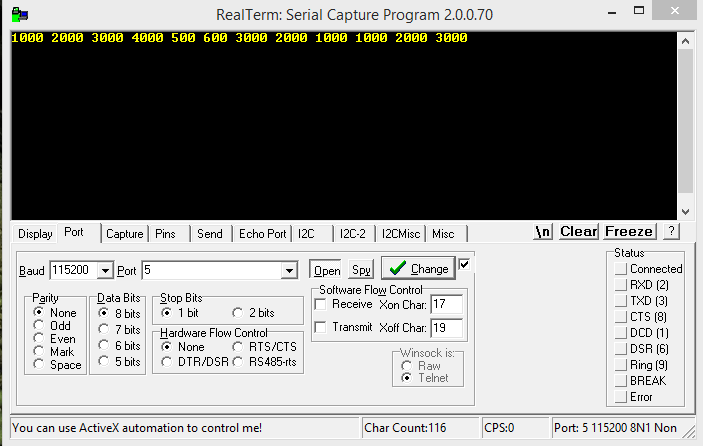
\includegraphics[width=0.8\textwidth]{./BluetoothWynikiNaTerminalu.PNG}
\caption{Bluetooth - wyniki na terminalu}
\label{fig:bluetooth}
\end{figure}
\subsection{Odczyt danych z czujników}
\subsubsection{Tensometry} \label{tensometry}
Dane z czujników są odczytywane za pomocą przetwornika ADC oraz przy użyciu DMA (Direct Memory Access), co pozwala na bezpośrednie przekierowanie danych z czujników do odpowiednich zmiennych, bez wywoływania dodatkowej funkcji zwracającej wynik pomiaru.
\subsubsection{Czujniki nacisku}
Obsługa taka sama jak w: \nameref{tensometry}.
\subsubsection{Akcelerometr}
Z akcelerometrem komunikacja następuje po interfejsie I2C.

\subsection{Rękawica sensoryczna}
Rękawica zbiera dane z trzech palców prawej ręki. Przyszyto 5 czujników ugięcia na zewnętrznej stronie dłoni, jeden wewnątrz [rys.  \ref{fig:rekawica2}]. Przetestowano kilka ustawień czujników i takie [rys.  \ref{fig:rekawica}] zdaje się najlepiej spełniać założenia, czyli poprawnie odczytywać zgięcia konkretnych stawów palców, nie ograniczając przy tym ruchów dłoni. Czujniki nacisku przymocowano na opuszkach. Zostały one przyklejone klejem błyskawicznym. Przymocowano również na wierzchu dłoni 2 listwy żeńskie do wpięcia płytki Discovery F3, aby móc pobierać dane z akcelerometru i wykrywać obrót ręki.
\begin{figure}[h]
\centering
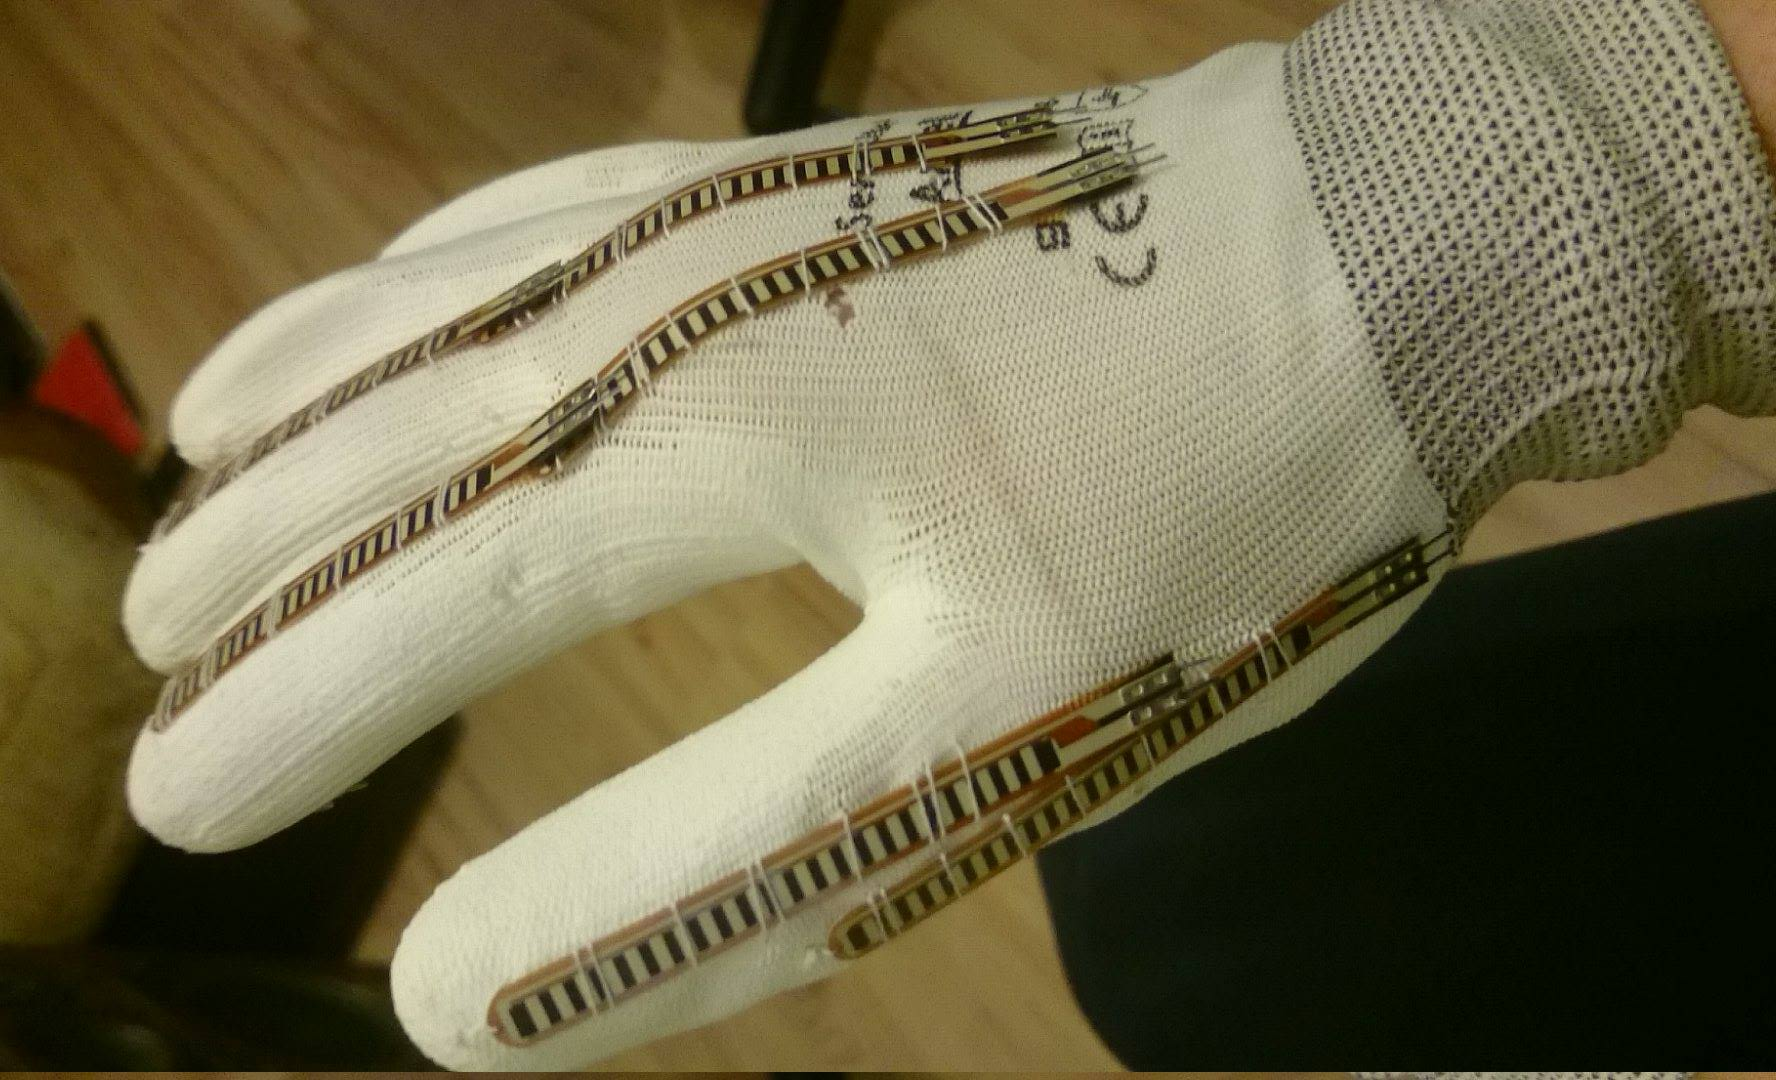
\includegraphics[width=0.8\textwidth]{./rekawica2.jpg}
\caption{Zdjęcie rękawicy}
\label{fig:rekawica2}
\end{figure}
\begin{figure}[h]
\centering
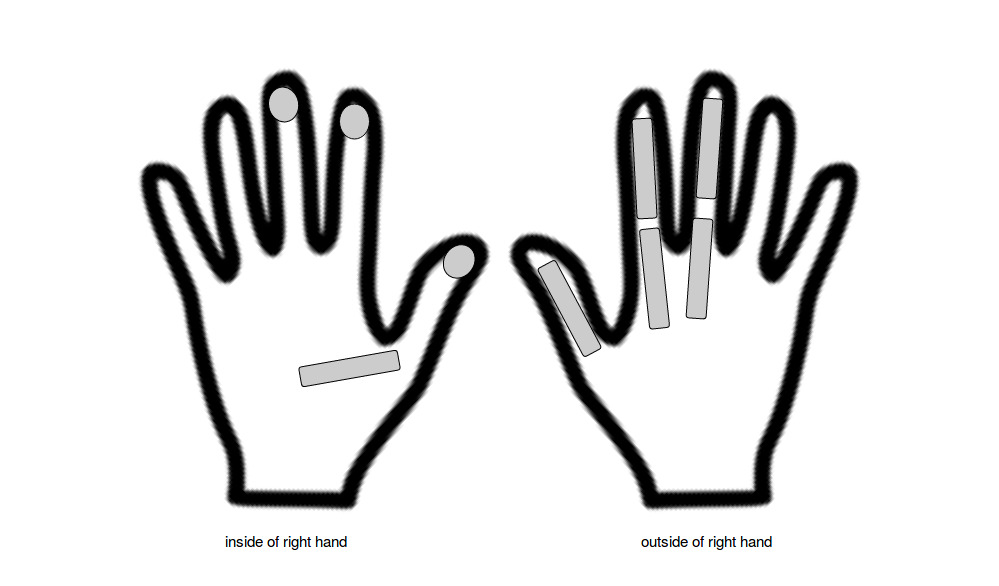
\includegraphics[width=1\textwidth]{./rekawica.jpg}
\caption{Schemat rozłożenia czujników}
\label{fig:rekawica}
\end{figure}

\section{Podsumowanie}
Większość prac została ukończona. Pozostało dopracowanie prototypu rękawicy i przeprowadzenie testów w celu zebrania pomiarów do bazy danych oraz wykonanie aplikacji pozwalającej na wizualizację modelu ręki na podstawie odczytów z czujników.

\end{document}
